%!TEX root = principal.tex
\chapter{Linguagem Grafcet}
O Grafcet pode ser definido em 2 níveis de abstração: o 1 e o 2. O nível 1 serve como uma ferramenta de desenvolvimento, para analisar a partir do problema como um todo a sequência de etapas, as ações a serem realizadas em cada etapa e as condições de transição de uma etapa para outra. No nível 1 as ações e transições são descritas de forma ampla, para permitirem uma melhor visualização do processo pelo desenvolvedor. O resultado final é uma descrição dos requisitos daquelas etapas e transições e não serve como uma linguagem para programar um sistema.

Já o Grafcet nível 2 é propriamente uma linguagem de programação, com diferentes implementações. Uma delas é o SFC - \emph{Sequential Function Chart}, descrita no padrão IEC1131-3 para programação de CLPs. No SFC, cada ação corresponde a uma atuação nas saídas ou variáveis internas do CLP e cada transição corresponde a um valor binário obtido no CLP seja de entradas, seja de comparações de valores analógicos ou de tempo.

Desta forma o principal uso do grafcet é num projeto top-down, onde a partir do problema se desenvolve a sequência a ser seguida no grafcet nível 1, a partir deste se definem todas as entradas, saídas e condições necessárias para o controle automático daquela sequência e então programa-se o sistema usando grafcet nível 2.

Tomemos como exemplo uma tarefa relativamente simples: cozinhar um ovo.

\begin{figure}[!h]
\centering
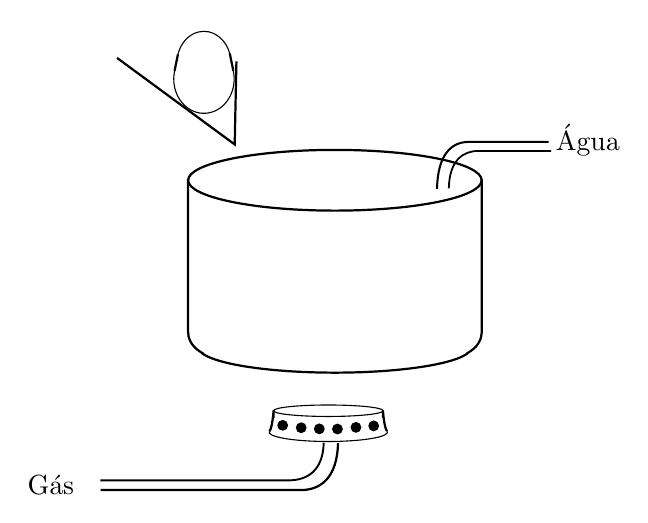
\begin{tikzpicture}[y=0.80pt, x=0.8pt,xscale=0.8,yscale=-0.8, inner sep=0pt, outer sep=0pt]
\begin{scope}[shift={(-99.03245,-288.02393)}]
    \path[draw=black,line join=miter,line cap=butt,line width=0.800pt]
      (354.2857,372.3622) .. controls (354.2857,381.8299) and (317.1893,389.5050) ..
      (271.4286,389.5050) .. controls (225.6678,389.5050) and (188.5714,381.8299) ..
      (188.5714,372.3622) .. controls (188.5714,362.8944) and (225.6678,355.2193) ..
      (271.4286,355.2193) .. controls (317.1893,355.2193) and (354.2857,362.8944) ..
      (354.2857,372.3622) -- cycle;
    \path[cm={{0.93174,0.0,0.0,0.83675,(18.52752,155.07504)}},draw=black,line
      join=miter,line cap=butt,line width=0.800pt] (351.5135,376.7594) .. controls
      (339.7757,385.9104) and (294.4050,391.3600) .. (250.1753,388.9315) .. controls
      (220.3437,387.2935) and (197.3850,382.3608) .. (190.5989,376.1313);
    \path[draw=black,line join=miter,line cap=butt,line width=0.800pt]
      (188.4845,371.6696) .. controls (188.4845,371.6696) and (188.4845,450.0421) ..
      (188.4845,457.6107) .. controls (188.4845,461.2730) and (190.0955,465.6973) ..
      (194.9956,468.8884) .. controls (198.4879,471.1627) and (197.0297,470.3066) ..
      (197.0297,470.3066);
    \path[draw=black,line join=miter,line cap=butt,line width=0.800pt]
      (354.3736,371.7266) .. controls (354.3736,371.7266) and (354.3736,450.0990) ..
      (354.3736,457.6677) .. controls (354.3736,461.3300) and (352.7625,465.7543) ..
      (347.8624,468.9454) .. controls (344.3701,471.2196) and (345.8283,470.3635) ..
      (345.8283,470.3635);
  \path[draw=black,line join=miter,line cap=butt,line width=0.800pt]
    (148.4437,303.3074) -- (214.8527,352.1376) -- (215.8294,305.2606);
  \begin{scope}[cm={{0.52126,0.0,0.0,0.55799,(132.31437,-4.68415)}}]
    \path[shift={(-3.38483,0)},draw=black] (160.1446,564.8529) .. controls
      (164.5668,583.4180) and (153.9497,602.2669) .. (136.4306,606.9532) .. controls
      (118.9114,611.6395) and (101.1244,600.3885) .. (96.7021,581.8235) .. controls
      (95.2554,575.7501) and (95.3885,569.3749) .. (97.0871,563.3753);
    \path[cm={{0.89621,0.0,0.0,-0.93321,(9.92999,1092.4228)}},draw=black]
      (160.3532,580.8939) .. controls (156.4154,599.5810) and (138.9277,611.3472) ..
      (121.2933,607.1743) .. controls (108.9462,604.2525) and (99.2953,594.0489) ..
      (96.5099,580.9713);
    \path[draw=black,line join=miter,line cap=butt,line width=0.800pt]
      (93.2329,565.0164) -- (96.8536,548.3611);
    \path[draw=black,line join=miter,line cap=butt,line width=0.800pt]
      (156.8450,565.0164) -- (153.0433,547.4560);
  \end{scope}
  \begin{scope}[shift={(0,10.0)}]
    \path[shift={(165.51847,-28.86265)},draw=black] (133.1216,521.3483) .. controls
      (133.1216,523.1376) and (119.2763,524.5880) .. (102.1973,524.5880) .. controls
      (85.1183,524.5880) and (71.2731,523.1376) .. (71.2731,521.3483) .. controls
      (71.2731,519.5591) and (85.1183,518.1086) .. (102.1973,518.1086) .. controls
      (119.2763,518.1086) and (133.1216,519.5591) .. (133.1216,521.3483) -- cycle;
    \path[cm={{0.95437,0.0,0.0,1.00307,(10.48141,-1.55578)}},draw=black]
      (304.2515,503.8934) .. controls (306.6885,506.7980) and (293.0976,509.4514) ..
      (273.8954,509.8200) .. controls (254.6932,510.1886) and (237.1512,508.1328) ..
      (234.7143,505.2283) .. controls (234.3214,504.7600) and (234.3437,504.2859) ..
      (234.7807,503.8186);
    \path[draw=black,line join=miter,line cap=butt,line width=0.800pt]
      (234.4953,503.9994) .. controls (236.1212,502.2258) and (236.7863,492.5444) ..
      (236.7863,492.5444) .. controls (236.7863,492.5444) and (236.7863,501.7823) ..
      (236.7863,492.2488);
    \path[draw=black,line join=miter,line cap=butt,line width=0.800pt]
      (300.8602,503.9994) .. controls (299.2343,502.2258) and (298.5692,492.5444) ..
      (298.5692,492.5444) .. controls (298.5692,492.5444) and (298.5692,501.7823) ..
      (298.5692,492.2488);
    \path[shift={(37.28111,-18.91723)},draw=black,fill=black] (248.7459,520.7984) ..
      controls (248.7459,522.2992) and (247.5293,523.5158) .. (246.0286,523.5158) ..
      controls (244.5278,523.5158) and (243.3112,522.2992) .. (243.3112,520.7984) ..
      controls (243.3112,519.2976) and (244.5278,518.0810) .. (246.0286,518.0810) ..
      controls (247.5293,518.0810) and (248.7459,519.2976) .. (248.7459,520.7984) --
      cycle;
    \path[shift={(26.8373,-17.9766)},draw=black,fill=black] (248.7459,520.7984) ..
      controls (248.7459,522.2992) and (247.5293,523.5158) .. (246.0286,523.5158) ..
      controls (244.5278,523.5158) and (243.3112,522.2992) .. (243.3112,520.7984) ..
      controls (243.3112,519.2976) and (244.5278,518.0810) .. (246.0286,518.0810) ..
      controls (247.5293,518.0810) and (248.7459,519.2976) .. (248.7459,520.7984) --
      cycle;
    \path[shift={(16.60251,-18.08111)},draw=black,fill=black] (248.7459,520.7984) ..
      controls (248.7459,522.2992) and (247.5293,523.5158) .. (246.0286,523.5158) ..
      controls (244.5278,523.5158) and (243.3112,522.2992) .. (243.3112,520.7984) ..
      controls (243.3112,519.2976) and (244.5278,518.0810) .. (246.0286,518.0810) ..
      controls (247.5293,518.0810) and (248.7459,519.2976) .. (248.7459,520.7984) --
      cycle;
    \path[shift={(6.36773,-18.7082)},draw=black,fill=black] (248.7459,520.7984) ..
      controls (248.7459,522.2992) and (247.5293,523.5158) .. (246.0286,523.5158) ..
      controls (244.5278,523.5158) and (243.3112,522.2992) .. (243.3112,520.7984) ..
      controls (243.3112,519.2976) and (244.5278,518.0810) .. (246.0286,518.0810) ..
      controls (247.5293,518.0810) and (248.7459,519.2976) .. (248.7459,520.7984) --
      cycle;
    \path[shift={(-4.07609,-20.0669)},draw=black,fill=black] (248.7459,520.7984) ..
      controls (248.7459,522.2992) and (247.5293,523.5158) .. (246.0286,523.5158) ..
      controls (244.5278,523.5158) and (243.3112,522.2992) .. (243.3112,520.7984) ..
      controls (243.3112,519.2976) and (244.5278,518.0810) .. (246.0286,518.0810) ..
      controls (247.5293,518.0810) and (248.7459,519.2976) .. (248.7459,520.7984) --
      cycle;
    \path[shift={(47.30687,-19.75335)},draw=black,fill=black] (248.7459,520.7984) ..
      controls (248.7459,522.2992) and (247.5293,523.5158) .. (246.0286,523.5158) ..
      controls (244.5278,523.5158) and (243.3112,522.2992) .. (243.3112,520.7984) ..
      controls (243.3112,519.2976) and (244.5278,518.0810) .. (246.0286,518.0810) ..
      controls (247.5293,518.0810) and (248.7459,519.2976) .. (248.7459,520.7984) --
      cycle;
  \end{scope}
  \path[draw=black,line join=miter,line cap=butt,line width=0.800pt]
    (273.1769,520.7233) .. controls (272.7485,540.4295) and (263.3238,547.2838) ..
    (252.1855,547.2838) .. controls (241.0472,547.2838) and (139.0890,547.2838) ..
    (139.0890,547.2838);
  \path[draw=black,line join=miter,line cap=butt,line width=0.692pt]
    (265.1049,520.6557) .. controls (264.7021,536.3302) and (255.8400,541.7823) ..
    (245.3666,541.7823) .. controls (234.8932,541.7823) and (139.0214,541.7823) ..
    (139.0214,541.7823);
  \path[fill=black] (97.967995,549.99866) node[above right] (text3077) {Gás};
  \path[draw=black,line join=miter,line cap=butt,line width=0.736pt]
    (329.0890,377.2838) .. controls (329.4517,357.5776) and (337.4309,350.7233) ..
    (346.8607,350.7233) .. controls (356.2906,350.7233) and (392.0864,350.7233) ..
    (392.0864,350.7233);
  \path[draw=black,line join=miter,line cap=butt,line width=0.638pt]
    (335.7362,376.9255) .. controls (336.0789,361.2509) and (343.6164,355.7989) ..
    (352.5243,355.7989) .. controls (361.4323,355.7989) and (393.4609,355.7989) ..
    (393.4609,355.7989);
  \path[fill=black] (396.19095,358.56888) node[above right] (text3085) {Água};
\end{scope}

\end{tikzpicture}
\caption{Sistema para cozinhar ovo sem sensores ou atuadores.}
\label{fig:cozinhar_ovo}
\end{figure}

\begin{figure}[!h]
\centering
\begin{tikzpicture}[scale=0.4]
\EtapeInit[0,0]{0}\ActionX{X0}{Esperando início.}
\Transition[VX0]{1}\Recept{T1}{Botão iniciar apertado e panela presente.}
\Etape[VT1]{1}\ActionX{X1}{Encher de água.}
\Transition{2}\Recept{T2}{Panela cheia}
\Etape[VT2]{2}\ActionX{X2}{Colocar o ovo}
\DivOU{X2}{18/L2,-3/L1}
\Transition[L1]{3}\Recept{T3}{Ovo presente.}
\Transition[L2]{7}\Recept{T7}{Ovo não presente.}
\DecaleNoeudx[-2]{T3}{T3f}
\DecaleNoeudx[-2]{VT3}{VT3f}
\ConvOU{T3f}{T3}{L11}
\Etape[L11]{3}\ActionX{X3}{Acionar o fogo.}
\DivOU{X3}{0/L6,12/L7}
\Transition[L6]{4}\Recept{T4}{Ovo cozido.}
\Transition[L7]{9}\Recept{T9}{Problema com o fogo.}
\ConvOU{T9}{T7}{L5}
\Etape[L5]{5}\ActionX{X5}{Deu bronca.}
\DivOU{X5}{0/L4,-7/L3}
\Transition[L3]{6}\Recept{T6}{Resolvido.}
\LienRetour[12]{T6}{VT3f}

\Transition[L4]{8}\Recept{T8}{Cancelado.}
%\LienRetour[-14]{T8}{X0}
\Etape[VT4]{4}\ActionX{X4}{Ovo pronto.}
\Transition[VX4]{5}\Recept{T5}{Panela retirada}
\LienTE[4]{T8}
\DecaleNoeudy[2]{T8}{T8}
\ConvOU{T8}{T5}{L9}
\LienTE[-4]{L9}
\LienRetour[-22]{L9}{X0}
 
 
% \LienRetour{T7}{X0}
\end{tikzpicture}
\caption{Diagrama grafcet nível 1 para cozinhar um ovo.}
\label{fig:grafcet1}
\end{figure}

\begin{figure}[!h]
\centering
\definecolor{c0000ff}{RGB}{0,0,255}
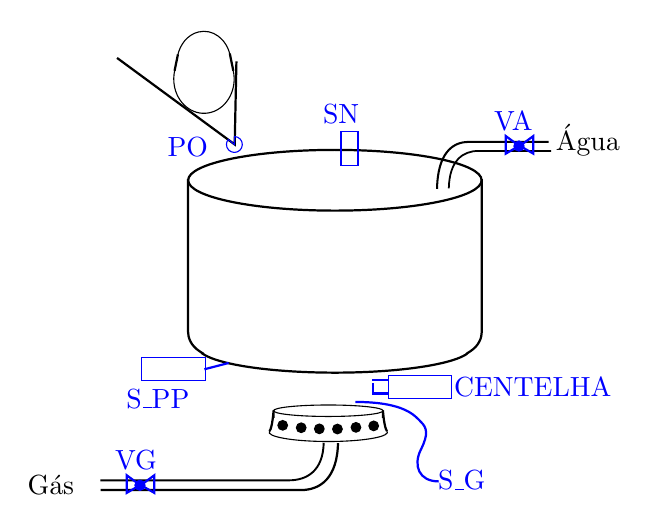
\begin{tikzpicture}[y=0.80pt, x=0.8pt,yscale=-0.8, xscale=0.8, inner sep=0pt, outer sep=0pt]
\begin{scope}[shift={(-99.03245,-288.02393)}]
    \path[draw=black,line join=miter,line cap=butt,line width=0.800pt]
      (354.2857,372.3622) .. controls (354.2857,381.8299) and (317.1893,389.5050) ..
      (271.4286,389.5050) .. controls (225.6678,389.5050) and (188.5714,381.8299) ..
      (188.5714,372.3622) .. controls (188.5714,362.8944) and (225.6678,355.2193) ..
      (271.4286,355.2193) .. controls (317.1893,355.2193) and (354.2857,362.8944) ..
      (354.2857,372.3622) -- cycle;
    \path[cm={{0.93174,0.0,0.0,0.83675,(18.52752,155.07504)}},draw=black,line
      join=miter,line cap=butt,line width=0.800pt] (351.5135,376.7594) .. controls
      (339.7757,385.9104) and (294.4050,391.3600) .. (250.1753,388.9315) .. controls
      (220.3437,387.2935) and (197.3850,382.3608) .. (190.5989,376.1313);
    \path[draw=black,line join=miter,line cap=butt,line width=0.800pt]
      (188.4845,371.6696) .. controls (188.4845,371.6696) and (188.4845,450.0421) ..
      (188.4845,457.6107) .. controls (188.4845,461.2730) and (190.0955,465.6973) ..
      (194.9956,468.8884) .. controls (198.4879,471.1627) and (197.0297,470.3066) ..
      (197.0297,470.3066);
    \path[draw=black,line join=miter,line cap=butt,line width=0.800pt]
      (354.3736,371.7266) .. controls (354.3736,371.7266) and (354.3736,450.0990) ..
      (354.3736,457.6677) .. controls (354.3736,461.3300) and (352.7625,465.7543) ..
      (347.8624,468.9454) .. controls (344.3701,471.2196) and (345.8283,470.3635) ..
      (345.8283,470.3635);
  \path[draw=black,line join=miter,line cap=butt,line width=0.800pt]
    (148.4437,303.3074) -- (214.8527,352.1376) -- (215.8294,305.2606);
  \begin{scope}[cm={{0.52126,0.0,0.0,0.55799,(132.31437,-4.68415)}}]
    \path[shift={(-3.38483,0)},draw=black] (160.1446,564.8529) .. controls
      (164.5668,583.4180) and (153.9497,602.2669) .. (136.4306,606.9532) .. controls
      (118.9114,611.6395) and (101.1244,600.3885) .. (96.7021,581.8235) .. controls
      (95.2554,575.7501) and (95.3885,569.3749) .. (97.0871,563.3753);
    \path[cm={{0.89621,0.0,0.0,-0.93321,(9.92999,1092.4228)}},draw=black]
      (160.3532,580.8939) .. controls (156.4154,599.5810) and (138.9277,611.3472) ..
      (121.2933,607.1743) .. controls (108.9462,604.2525) and (99.2953,594.0489) ..
      (96.5099,580.9713);
    \path[draw=black,line join=miter,line cap=butt,line width=0.800pt]
      (93.2329,565.0164) -- (96.8536,548.3611);
    \path[draw=black,line join=miter,line cap=butt,line width=0.800pt]
      (156.8450,565.0164) -- (153.0433,547.4560);
  \end{scope}
  \begin{scope}[shift={(0,10.0)}]
    \path[shift={(165.51847,-28.86265)},draw=black] (133.1216,521.3483) .. controls
      (133.1216,523.1376) and (119.2763,524.5880) .. (102.1973,524.5880) .. controls
      (85.1183,524.5880) and (71.2731,523.1376) .. (71.2731,521.3483) .. controls
      (71.2731,519.5591) and (85.1183,518.1086) .. (102.1973,518.1086) .. controls
      (119.2763,518.1086) and (133.1216,519.5591) .. (133.1216,521.3483) -- cycle;
    \path[cm={{0.95437,0.0,0.0,1.00307,(10.48141,-1.55578)}},draw=black]
      (304.2515,503.8934) .. controls (306.6885,506.7980) and (293.0976,509.4514) ..
      (273.8954,509.8200) .. controls (254.6932,510.1886) and (237.1512,508.1328) ..
      (234.7143,505.2283) .. controls (234.3214,504.7600) and (234.3437,504.2859) ..
      (234.7807,503.8186);
    \path[draw=black,line join=miter,line cap=butt,line width=0.800pt]
      (234.4953,503.9994) .. controls (236.1212,502.2258) and (236.7863,492.5444) ..
      (236.7863,492.5444) .. controls (236.7863,492.5444) and (236.7863,501.7823) ..
      (236.7863,492.2488);
    \path[draw=black,line join=miter,line cap=butt,line width=0.800pt]
      (300.8602,503.9994) .. controls (299.2343,502.2258) and (298.5692,492.5444) ..
      (298.5692,492.5444) .. controls (298.5692,492.5444) and (298.5692,501.7823) ..
      (298.5692,492.2488);
    \path[shift={(37.28111,-18.91723)},draw=black,fill=black] (248.7459,520.7984) ..
      controls (248.7459,522.2992) and (247.5293,523.5158) .. (246.0286,523.5158) ..
      controls (244.5278,523.5158) and (243.3112,522.2992) .. (243.3112,520.7984) ..
      controls (243.3112,519.2976) and (244.5278,518.0810) .. (246.0286,518.0810) ..
      controls (247.5293,518.0810) and (248.7459,519.2976) .. (248.7459,520.7984) --
      cycle;
    \path[shift={(26.8373,-17.9766)},draw=black,fill=black] (248.7459,520.7984) ..
      controls (248.7459,522.2992) and (247.5293,523.5158) .. (246.0286,523.5158) ..
      controls (244.5278,523.5158) and (243.3112,522.2992) .. (243.3112,520.7984) ..
      controls (243.3112,519.2976) and (244.5278,518.0810) .. (246.0286,518.0810) ..
      controls (247.5293,518.0810) and (248.7459,519.2976) .. (248.7459,520.7984) --
      cycle;
    \path[shift={(16.60251,-18.08111)},draw=black,fill=black] (248.7459,520.7984) ..
      controls (248.7459,522.2992) and (247.5293,523.5158) .. (246.0286,523.5158) ..
      controls (244.5278,523.5158) and (243.3112,522.2992) .. (243.3112,520.7984) ..
      controls (243.3112,519.2976) and (244.5278,518.0810) .. (246.0286,518.0810) ..
      controls (247.5293,518.0810) and (248.7459,519.2976) .. (248.7459,520.7984) --
      cycle;
    \path[shift={(6.36773,-18.7082)},draw=black,fill=black] (248.7459,520.7984) ..
      controls (248.7459,522.2992) and (247.5293,523.5158) .. (246.0286,523.5158) ..
      controls (244.5278,523.5158) and (243.3112,522.2992) .. (243.3112,520.7984) ..
      controls (243.3112,519.2976) and (244.5278,518.0810) .. (246.0286,518.0810) ..
      controls (247.5293,518.0810) and (248.7459,519.2976) .. (248.7459,520.7984) --
      cycle;
    \path[shift={(-4.07609,-20.0669)},draw=black,fill=black] (248.7459,520.7984) ..
      controls (248.7459,522.2992) and (247.5293,523.5158) .. (246.0286,523.5158) ..
      controls (244.5278,523.5158) and (243.3112,522.2992) .. (243.3112,520.7984) ..
      controls (243.3112,519.2976) and (244.5278,518.0810) .. (246.0286,518.0810) ..
      controls (247.5293,518.0810) and (248.7459,519.2976) .. (248.7459,520.7984) --
      cycle;
    \path[shift={(47.30687,-19.75335)},draw=black,fill=black] (248.7459,520.7984) ..
      controls (248.7459,522.2992) and (247.5293,523.5158) .. (246.0286,523.5158) ..
      controls (244.5278,523.5158) and (243.3112,522.2992) .. (243.3112,520.7984) ..
      controls (243.3112,519.2976) and (244.5278,518.0810) .. (246.0286,518.0810) ..
      controls (247.5293,518.0810) and (248.7459,519.2976) .. (248.7459,520.7984) --
      cycle;
  \end{scope}
  \path[draw=black,line join=miter,line cap=butt,line width=0.800pt]
    (273.1769,520.7233) .. controls (272.7485,540.4295) and (263.3238,547.2838) ..
    (252.1855,547.2838) .. controls (241.0472,547.2838) and (139.0890,547.2838) ..
    (139.0890,547.2838);
  \path[draw=black,line join=miter,line cap=butt,line width=0.692pt]
    (265.1049,520.6557) .. controls (264.7021,536.3302) and (255.8400,541.7823) ..
    (245.3666,541.7823) .. controls (234.8932,541.7823) and (139.0214,541.7823) ..
    (139.0214,541.7823);
  \path[fill=black] (97.967995,549.99866) node[above right] (text3077) {Gás};
  \path[draw=black,line join=miter,line cap=butt,line width=0.736pt]
    (329.0890,377.2838) .. controls (329.4517,357.5776) and (337.4309,350.7233) ..
    (346.8607,350.7233) .. controls (356.2906,350.7233) and (392.0864,350.7233) ..
    (392.0864,350.7233);
  \path[draw=black,line join=miter,line cap=butt,line width=0.638pt]
    (335.7362,376.9255) .. controls (336.0789,361.2509) and (343.6164,355.7989) ..
    (352.5243,355.7989) .. controls (361.4323,355.7989) and (393.4609,355.7989) ..
    (393.4609,355.7989);
  \path[fill=black] (396.19095,358.56888) node[above right] (text3085) {Água};
  \path[draw=c0000ff,rounded corners=0.0000cm] (274.8555,344.6107) rectangle
    (284.4550,363.8097);
  \path[text=c0000ff] (264.7507,340.06354) node[above right] (text3091) {SN};
  \path[shift={(103.79863,289.84629)},draw=c0000ff] (111.0562,57.8371) .. controls
    (113.5319,57.9323) and (115.4616,60.0164) .. (115.3663,62.4920) .. controls
    (115.2711,64.9676) and (113.1870,66.8973) .. (110.7114,66.8021) .. controls
    (108.2358,66.7069) and (106.3061,64.6228) .. (106.4013,62.1472) .. controls
    (106.4392,61.1629) and (106.8000,60.2184) .. (107.4280,59.4596) --
    (110.8838,62.3196) -- cycle;
  \path[text=c0000ff] (176.97354,359.03479) node[above right] (text3097) {PO};
  \path[shift={(99.03245,288.02393)},draw=c0000ff,rounded corners=0.0000cm]
    (63.3622,184.2778) rectangle (99.2487,197.1745);
  \path[shift={(99.03245,288.02393)},draw=c0000ff,line join=miter,line
    cap=butt,line width=0.800pt] (98.7270,191.0482) .. controls
    (112.6043,187.4797) and (112.4061,187.4797) .. (112.4061,187.4797);
  \path[text=c0000ff] (153.71358,501.07755) node[above right] (text3105) {S\_PP};
  \begin{scope}[shift={(-4.37896,11.89482)}]
    \path[shift={(109.53954,277.51684)},draw=c0000ff,fill=c0000ff]
      (59.0776,255.1811) .. controls (59.0776,256.7687) and (57.7906,258.0557) ..
      (56.2030,258.0557) .. controls (54.6154,258.0557) and (53.3285,256.7687) ..
      (53.3285,255.1811) .. controls (53.3285,253.5935) and (54.6154,252.3065) ..
      (56.2030,252.3065) .. controls (57.7906,252.3065) and (59.0776,253.5935) ..
      (59.0776,255.1811) -- cycle;
    \path[shift={(99.03245,288.02393)},draw=c0000ff,line join=miter,line
      cap=butt,line width=0.800pt] (66.8093,244.5749) -- (59.2477,248.9406) --
      (59.2477,239.0240) -- cycle;
    \path[draw=c0000ff,line join=miter,line cap=butt,line width=0.800pt]
      (166.2801,532.5988) -- (173.8417,536.9645) -- (173.8417,527.0479) -- cycle;
  \end{scope}
  \path[text=c0000ff] (147.31708,535.6076) node[above right] (text3122) {VG};
  \begin{scope}[shift={(209.61758,-179.63899)}]
    \path[shift={(109.53954,277.51684)},draw=c0000ff,fill=c0000ff]
      (59.0776,255.1811) .. controls (59.0776,256.7687) and (57.7906,258.0557) ..
      (56.2030,258.0557) .. controls (54.6154,258.0557) and (53.3285,256.7687) ..
      (53.3285,255.1811) .. controls (53.3285,253.5935) and (54.6154,252.3065) ..
      (56.2030,252.3065) .. controls (57.7906,252.3065) and (59.0776,253.5935) ..
      (59.0776,255.1811) -- cycle;
    \path[shift={(99.03245,288.02393)},draw=c0000ff,line join=miter,line
      cap=butt,line width=0.800pt] (66.8093,244.5749) -- (59.2477,248.9406) --
      (59.2477,239.0240) -- cycle;
    \path[draw=c0000ff,line join=miter,line cap=butt,line width=0.800pt]
      (166.2801,532.5988) -- (173.8417,536.9645) -- (173.8417,527.0479) -- cycle;
  \end{scope}
  \path[text=c0000ff] (361.31363,344.07382) node[above right] (text3122-9) {VA};
  \path[draw=c0000ff,line join=miter,line cap=butt,line width=0.800pt]
    (282.9510,497.5344) .. controls (310.9874,497.5344) and (316.5946,505.3846) ..
    (319.9590,508.7490) .. controls (323.3234,512.1133) and (324.4448,515.4777) ..
    (319.9590,524.4493) .. controls (315.4732,533.4210) and (318.8376,542.3926) ..
    (330.0521,542.3926);
  \path[text=c0000ff] (329.78195,547.05719) node[above right] (text3161) {S\_G};
  \path[draw=c0000ff,rounded corners=0.0000cm] (301.4550,482.6751) rectangle
    (337.3415,495.5719);
  \path[text=c0000ff] (338.7536,494.34882) node[above right] (text3183) {CENTELHA};
  \path[shift={(99.03245,288.02393)},draw=c0000ff,line join=miter,line
    cap=butt,line width=0.800pt] (202.5627,204.7443) -- (193.7313,204.7443) --
    (193.7313,198.9969);
  \path[shift={(99.03245,288.02393)},draw=c0000ff,line join=miter,line
    cap=butt,line width=0.800pt] (202.2824,197.1745) -- (193.5911,197.1745);
\end{scope}

\end{tikzpicture}
\caption{Sistema para cozinhar ovo com sensores e atuadores.}
\label{fig:cozinhar_ovo2}
\end{figure}

\begin{figure}[!h]
{\centering
\begin{tikzpicture}[scale=0.4]
\EtapeInit[0,0]{0}%\ActionX{X0}{Esperando início.}
\Transition[VX0]{1}\Recept{T1}{B\_I \emph{AND} S\_PP}
\Etape[VT1]{1}\ActionX{X1}{VA}
\Transition{2}\Recept{T2}{SN<nivel\_agua\_ovo\_galinha}
\Etape[VT2]{2}\ActionX{X2}{PO}
\DivOU{X2}{18/L2,-3/L1}
\Transition[L1]{3}\Recept{T3}{A}
\Transition[L2]{7}\Recept{T7}{B}
\DecaleNoeudx[-2]{T3}{T3f}
\DecaleNoeudx[-2]{VT3}{VT3f}
\ConvOU{T3f}{T3}{L6}
\Etape[L6]{3a}\ActionX{X3a}{VG}
\DivOU{X3a}{0/L6a,19/L7a}
\Transition[L6a]{10}\Recept{T10}{SG}
\Transition[L7a]{11}\Recept{T11}{C}
\Etape[VT10]{3b}\ActionXV{X3b}{VG}\Action{X3b}{P}\Action{X3b}{CENTELHA}
\LienET[5]{X3b}
%\Etape[VT10]{3b}\ActionX{X3b}{VG}\Action{X3b}{P}\Action{X3b}{CENTELHA}
\DivOU{X3b}{0/L6,16/L7}
\Transition[L6]{4}\Recept{T4}{E}
\Transition[L7]{9}\Recept{T9}{D}
\ConvOU{T9}{T7,T11}{L5}
\Etape[L5]{5}\ActionX{X5}{A}
\DivOU{X5}{0/L4,-7/L3}
\Transition[L3]{6}\Recept{T6}{B\_OK}
\LienRetour[12]{T6}{VT3f}

\Transition[L4]{8}\Recept{T8}{B\_C}
%\LienRetour[-14]{T8}{X0}
\Etape[VT4]{4}%\ActionX{X4}{Ovo pronto.}
\Transition[VX4]{5}\Recept{T5}{\emph{AND} S\_PP}
\LienTE[4]{T8}
\DecaleNoeudy[2]{T8}{T8}
\ConvOU{T8}{T5}{L9}
\LienTE[-4]{L9}
\LienRetour[-14]{L9}{X0}
 
 
% \LienRetour{T7}{X0}
\end{tikzpicture}
}
A = S\_N < (nivel\_ovo\_galinha - volume\_ovo\_galinha)

B = \emph{NOT} A \emph{AND} 2.T>T\#10s

C = \emph{NOT} SG \emph{AND} 3a.T>T\#4s

D = SG \emph{AND} 3b.T>T\#4s

E = \emph{NOT} SG \emph{AND} 3b.T>tempo\_ovo\_galinha

\caption{Diagrama grafcet nível 2 para cozinhar um ovo.}
\label{fig:grafcet2}
\end{figure}

